\documentclass[a4paper,UTF8]{ctexart}

\usepackage{amsmath, amsthm, amssymb, amsfonts, hyperref, mathrsfs}%美国数学学会的包+?
\usepackage{geometry} %控制界面
\usepackage{bookmark}
\usepackage{fancyhdr} % header & footer
\usepackage{appendix} % 附录
\usepackage{tikz} %作图
\usepackage{graphicx} %插入图片的宏包
\usepackage{float} %设置图片浮动位置的宏包
\usepackage{subfigure} %插入多图时用子图显示的宏包
\usepackage{listings} %引用代码
\usepackage{physics,mathtools} %物理数学工具
\usepackage{framed}
\usepackage{comment}
\geometry{top=2.5cm,bottom=2.5cm,left=2.5cm,right=2.5cm} % 布局要求
\pagestyle{fancy} % fancy分格
\fancyhf{} % 清除所有页眉页脚
\renewcommand\headrulewidth{0.6pt}
\renewcommand\footrulewidth{0.6pt}
\lhead{何金铭 PB21020660$\mid$座位号:2}
\chead{单色仪的定标和光谱测量实验}
\rhead{\thepage}
\lfoot{2023.3.21}
\rfoot{USTC}
\bibliographystyle{plain} % 引用样式
%\bibliography{math}
\everymath{\displaystyle} % display
%============================================================

\begin{document}

\begin{center}
    \textbf{\Large 单色仪的定标和光谱测量实验}
    \par \text{\large 何金铭 PB21020660}
\end{center}

\begin{abstract}
    单色仪是指从一束电磁辐射中分离出波长范围极窄单色光的仪器,其在现代物理实验中起到重要的作用。本
    实验将利用光栅单色仪进行对钠灯光谱的测量,并由此计算里德伯常数;并且还会测量红宝石的发射光谱和吸收光谱。
    \par\textbf{关键词:}光栅单色仪,钠灯光谱,红宝石的发射与吸收光谱
\end{abstract}

\section{引言}
    光谱分析是现代物理学研究中经常会使用的方法,单色仪就是一种测量光谱的仪器,其可以从一束电磁辐射中分离出波长范围极窄单色光。
    单色仪有很多种类,其中最常用的就是光栅单色仪,由主要用到的原理有:闪耀光栅提取不同级数的衍射条纹的性质。再加之CCD和步进电机
    的精确控制,可以达到很高的精度和分辨本领。在本次实验中,将利用光栅单色仪进行对钠灯光谱的测量,并由此计算里德伯常数;并且还会测量红宝石的发射光谱和吸收光谱。
\section{实验仪器}

WDS-8型组合式多功能光栅光谱仪、低压钠灯、半导体激光器(532nm)、溴钨灯、红宝石、凸透镜、其他辅助仪器

\begin{comment}
\begin{enumerate}
    \item WDS-8型组合式多功能光栅光谱仪
    \item 低压钠灯
    \item 半导体激光器
    \item 溴钨灯
    \item 红宝石
    \item 凸透镜
\end{enumerate}
\end{comment}

\section{实验内容}

\subsection{光栅单色仪的定标}

\begin{figure}[H]
    \centering
    \begin{minipage}[b]{0.9\textwidth}
        \centering
        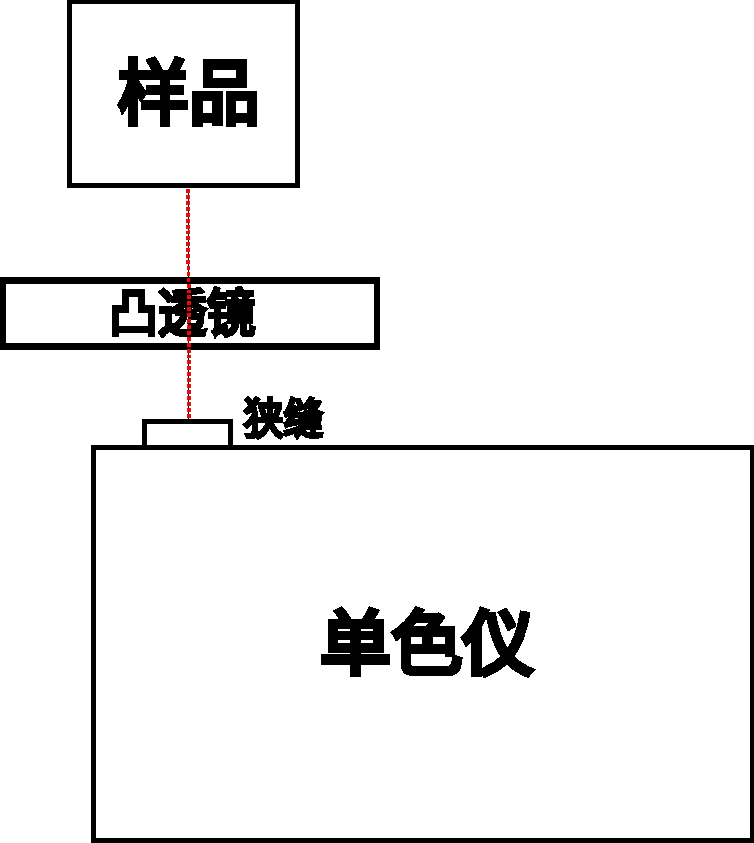
\includegraphics[width=0.4\textwidth]{./demo.pdf}
        \caption{实验光路}
    \end{minipage}
\end{figure}

实验开始前给单色仪定标,依照光路图搭建光路,测定钠灯主线系的光谱,比较其较大峰值和589nm的偏差,
按照差值对单色仪进行相应的标定。

在搭建实验光路时,要注意光路中的样品、凸透镜和狭缝需要在同一直线上,并且需要将样品成的像置于狭缝上,
其成清晰的缩小的实像。

\subsection{低压钠灯各个谱线系的光谱测量}

利用经标定的单色仪测量钠灯的各个谱线系,大致光路图同上,并据此计算里德伯常数。

不同线系有不同的计算公式:

\subsubsection{主线系}

\begin{equation}
    \frac{1}{\lambda} = R(\frac{1}{(3-\Delta s)^2}-\frac{1}{(3-\Delta p)^2}) , (\Delta s = 1.35,\Delta p = 0.86)
\end{equation}

\subsubsection{锐线系}

\begin{equation}
    \frac{1}{\lambda} = R(\frac{1}{(3-\Delta p)^2}-\frac{1}{(5-\Delta s)^2}) , (\Delta s = 1.35,\Delta p = 0.86)
\end{equation}

\subsubsection{漫线系}

\begin{equation}
    \frac{1}{\lambda} = R(\frac{1}{(3-\Delta p)^2}-\frac{1}{(n-\Delta d)^2}) , (n=4,5;\Delta d = 0.01,\Delta p = 0.86)
\end{equation}

\subsection{红宝石晶体的发射和吸收光谱的测量}

利用经标定的单色仪测量红宝石晶体的发射和吸收谱线,大致光路图同上,并分析红宝石晶体的发光原理和应用。

在搭建光路的时候,只需将红宝石放在狭缝之前较合适的距离即可,使得透射的像成于狭缝上。

于本文中,为了表述红宝石的吸收度,定义其值为$\frac{I_0}{I}$,其吸收曲线则为$\frac{I_0}{I}$-$\lambda$

吸收曲线不同于直接测量,故先测出入射光源(溴钨灯)的发射曲线,再测出经过红宝石的发射曲线,将两个曲线中的采样点数值相除
即可得到其吸收曲线。

\section{数据处理与分析}

\subsection{光栅单色仪的定标}

\begin{figure}[H]
    \centering
    \begin{minipage}[b]{0.9\textwidth}
        \centering
        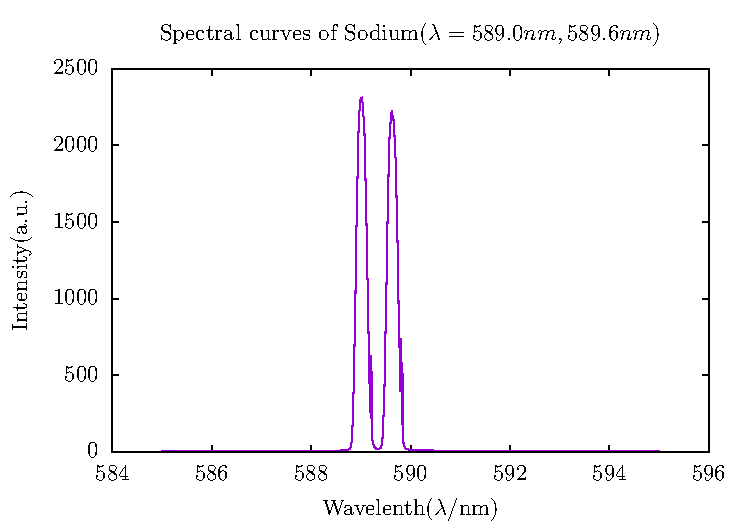
\includegraphics[width=0.7\textwidth]{./na_0.pdf}
        \caption{低压钠灯的主线系光谱}
    \end{minipage}
\end{figure}

测得的光谱如上,由实验测得的数据得其主线系峰值为590.025nm和596.025nm处。

\begin{table}[H]
    \centering
    \begin{tabular}{|c|c|c|c|}
    \hline
        $\lambda$(nm) & I(a.u.) & $\lambda$(nm) & I(a.u.) \\ \hline
        588.9875 & 2294 & 589.5875 & 2138 \\ 
        589.0000 & 2304 & 589.6000 & 2148 \\ 
        589.0125 & 2297 & 589.6125 & 2206 \\ 
        589.0250 & 2306 & 589.6250 & 2228 \\ 
        589.0375 & 2273 & 589.6375 & 2196 \\ \hline
    \end{tabular}
    \caption{钠灯主线系光谱部分数据}
\end{table}

但由于我们测得的光谱是取一些列的离散的采样点,所以其峰值应该处在一个区间范围之内,比如589nm附近的峰值,
其最可能的取值在588.9875nm和589.0375nm之间。而596nm附近的峰值则最可能在589.6125nm和589.6375之间。
而且可以发现,钠灯于589.0nm和589.025处的光强相差无几。

所以分析得:单色仪的波长检测功能基本正常,不需要进行定标(或者说处于定标的误差范围之内)。可以继续进行之后的实验。

并且,在之后的分析中,将不再像这里一样具体的分析峰值附近的数据,将直接给出相应的峰值。

\subsection{测量低压钠灯的光谱}

\subsubsection{主线系}

\begin{figure}[H]
    \centering
    \begin{minipage}[b]{0.9\textwidth}
        \centering
        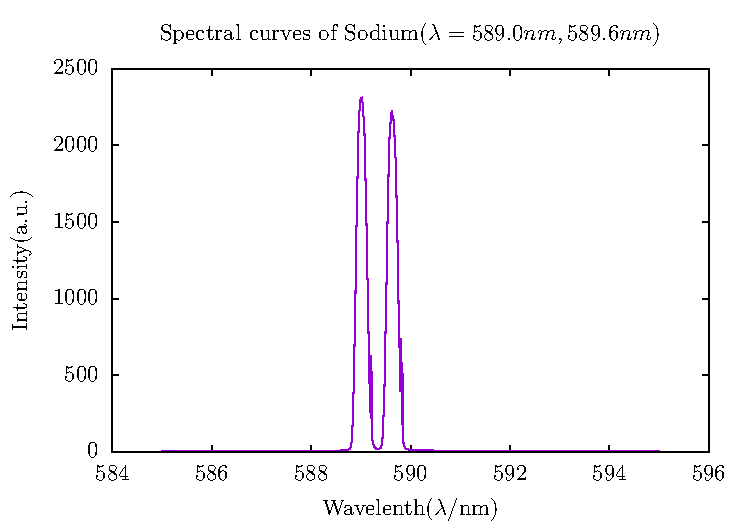
\includegraphics[width=0.7\textwidth]{./na_0.pdf}
        \caption{低压钠灯的主线系光谱}
    \end{minipage}
\end{figure}

此时的负高压为-385V。测得的光谱如上,其主线系峰值为590.025nm和596.025nm处。
其两个峰旁边均有一些毛刺,可能是由于宇宙线导致的。

由于两个峰强度近似相同,所以取平均波长$\lambda = 589.3025nm$代入主线系公式,得

\begin{equation}
    R = 1.13926 \times 10^7 m^{-1}
\end{equation}

\subsubsection{锐线系}

\begin{figure}[H]
    \centering
    \begin{minipage}[b]{0.9\textwidth}
        \centering
        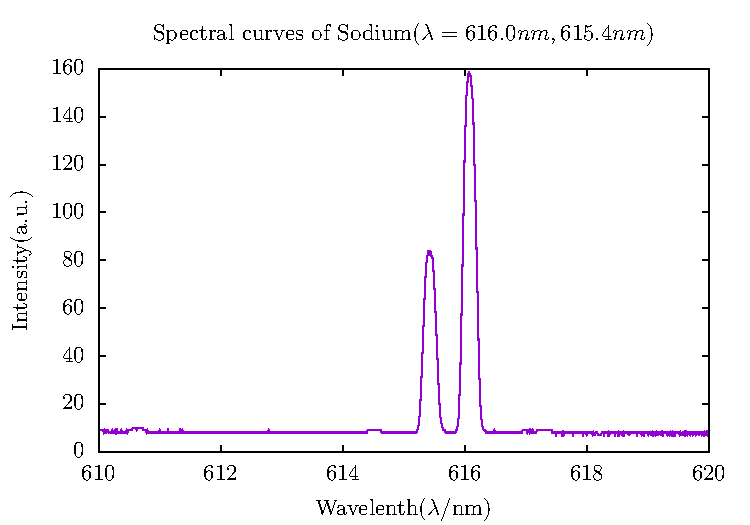
\includegraphics[width=0.7\textwidth]{./na_1.pdf}
        \caption{低压钠灯的锐线系光谱}
    \end{minipage}
\end{figure}

此时的负高压为-701V。测得的光谱如上,其锐线系峰值为615.4nm和616.075nm处。
锐线系的光强较弱,所以可以观察到背景光强,且其在不断的变化,代表着环境光强的改变。

观察得其两峰强度比为1:2,故波长数的比值也取为1:2,取平均波长$\lambda = 615.8nm$,
代入公式计算得:

\begin{equation}
    R = 1.13323 \times 10^7 m^{-1}
\end{equation}

\subsubsection{漫线系——谱线1}

\begin{figure}[H]
    \centering
    \begin{minipage}[b]{0.9\textwidth}
        \centering
        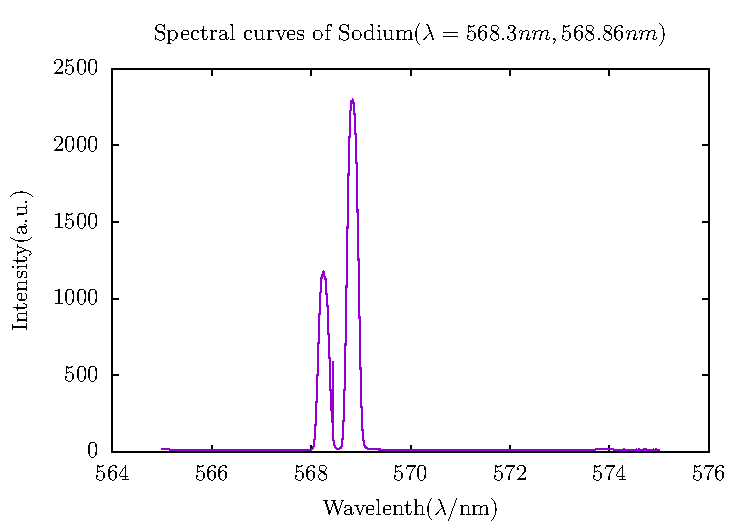
\includegraphics[width=0.7\textwidth]{./na_2.pdf}
        \caption{低压钠灯的漫线系光谱——谱线1}
    \end{minipage}
\end{figure}

此时的负高压为-803V。测得的光谱如上,其漫线系的第一个谱线的峰值为568.25nm和568.8375nm处。
其第一个峰旁边有毛刺,可能是由于宇宙线或者机械抖动导致的。

观察得其两峰强度比为1:2,故波长数的比值也取为1:2,取平均波长$\lambda = 568.64nm$,
代入公式计算得:

\begin{equation}
    R = 1.13286 \times 10^7 m^{-1}
\end{equation}

\subsubsection{漫线系——谱线2}

\begin{figure}[H]
    \centering
    \begin{minipage}[b]{0.9\textwidth}
        \centering
        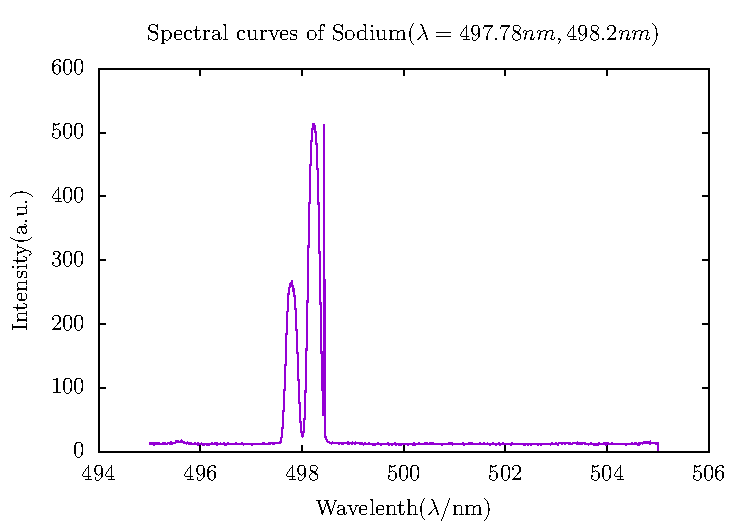
\includegraphics[width=0.8\textwidth]{./na_3.pdf}
        \caption{低压钠灯的漫线系光谱——谱线2}
    \end{minipage}
\end{figure}

此时的负高压为-853V。测得的光谱如上,其漫线系的第二个谱线的峰值为497.8nm和498.25nm处

另外观察到其中一条毛刺状的峰值,其只有一个采样点,推测为宇宙射线导致。

观察得其两峰强度比为1:2,故波长数的比值也取为1:2,取平均波长$\lambda = 498.1nm$,
代入公式计算得:

\begin{equation}
    R = 1.12662 \times 10^7 m^{-1}
\end{equation}

\subsubsection{分析计算得到里德伯常数的误差}

\begin{table}[H]
    \centering
    \begin{tabular}{|c|c|c|c|c|c|}
    \hline
        type & R & $R_{main}$ & $R_{sharp}$ & $R_{diffuse1}$ & $R_{diffuse2}$ \\ \hline
        $10^{7} m^{-1}$ & 1.09737 & 1.13926 & 1.13323 & 1.13286 & 1.12662 \\ \hline
    \end{tabular}
    \caption{里德伯常数对比}
\end{table}

发现测得的里德伯常数均大于实际的里德伯常数,最可能的原因是:理论模型存在考虑不完全的地方。由于测得的光谱与
国际上常用的标准值接近,但按所给公式计算出来仍有问题。另一方面,不同方法测得的里德伯常数不同,最可能的原因是
:各个理论模型间的偏差是不同的。

\subsection{红宝石晶体的发射和吸收光谱}

\subsubsection{红宝石晶体的发射光谱}

\begin{figure}[H]
    \centering
    \begin{minipage}[b]{0.9\textwidth}
        \centering
        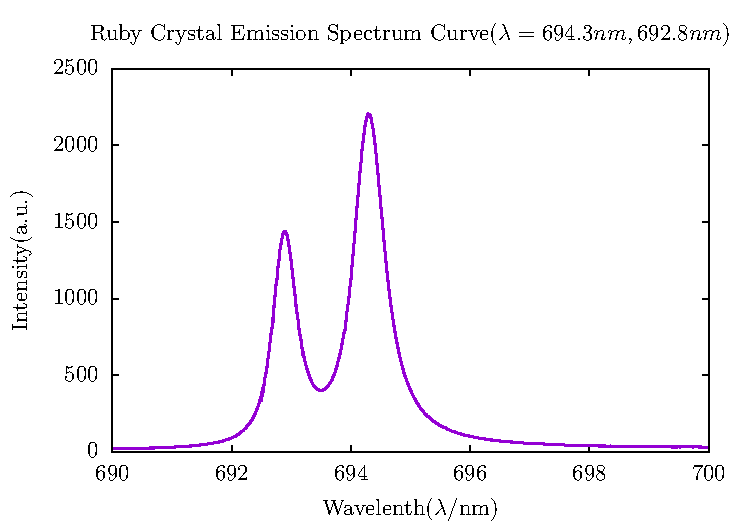
\includegraphics[width=0.7\textwidth]{./r_1.pdf}
        \caption{红宝石晶体的发射光谱}
    \end{minipage}
\end{figure}

此时的负高压为-663V。测得的光谱如上,发现红宝石的发射光谱中心位于692.875nm和694.2875nm处。
且694.2875nm处的光强度大于692.875nm处的光强度。

\subsubsection{溴钨灯的发射光谱}

\begin{figure}[H]
    \centering
    \begin{minipage}[b]{0.9\textwidth}
        \centering
        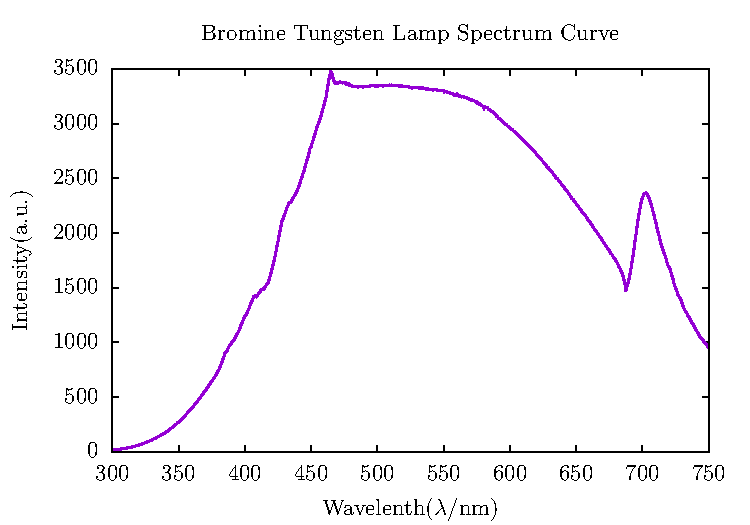
\includegraphics[width=0.8\textwidth]{./r_2.pdf}
        \caption{溴钨灯的发射光谱}
    \end{minipage}
\end{figure}

此时的负高压为-594V。

\subsubsection{通过红宝石晶体的溴钨灯的发射光谱}

\begin{figure}[H]
    \centering
    \begin{minipage}[b]{0.9\textwidth}
        \centering
        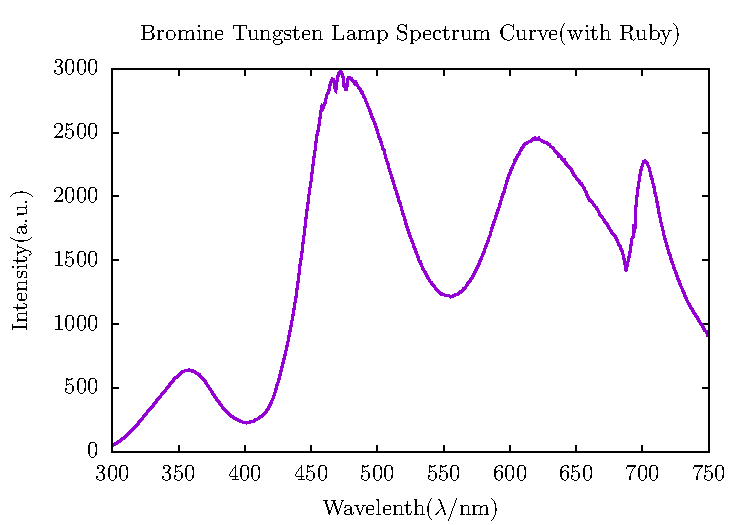
\includegraphics[width=0.7\textwidth]{./r_3.pdf}
        \caption{通过红宝石晶体的溴钨灯的发射光谱}
    \end{minipage}
\end{figure}

此时的负高压为-721V。

\subsubsection{红宝石晶体的吸收光谱}

\begin{figure}[H]
    \centering
    \begin{minipage}[b]{0.9\textwidth}
        \centering
        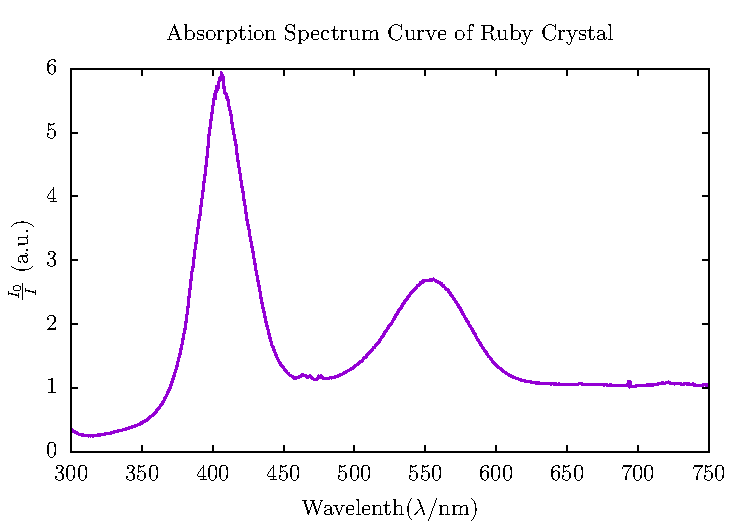
\includegraphics[width=0.7\textwidth]{./n_1.pdf}
        \caption{红宝石晶体的吸收光谱}
    \end{minipage}
\end{figure}

\begin{figure}[H]
    \centering
    \begin{minipage}[b]{0.9\textwidth}
        \centering
        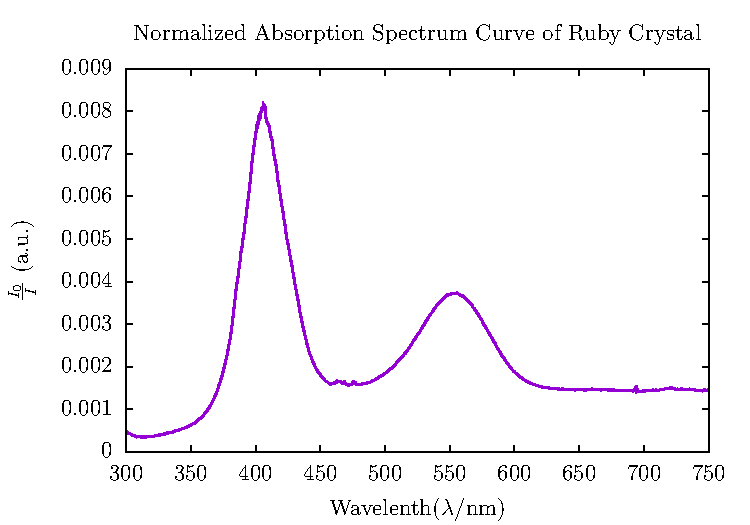
\includegraphics[width=0.7\textwidth]{./n_2.pdf}
        \caption{归一化后的红宝石晶体的吸收光谱}
    \end{minipage}
\end{figure}

直接读取数据,其吸收光谱的峰值中心位于406.2nm处和555.6nm处。
并且可以分析得到其带宽大致为100nm左右,且发现红宝石对紫外光的吸收弱于其对可光的吸收。

\subsubsection{红宝石晶体的发光原理以及应用}

以下内容部分参考此文献\cite{a}\cite{this}。

红宝石是掺有少量 Cr 的 $Al_2O_3$ 单晶,Cr 的外层电子组态为 $3d^54S^1$
,掺入 $Al_2O_3$
晶格后,失去外层三个电子,变成三价的 $Cr^{3+}$离子,红宝石晶体的光谱就是 $Cr^{3+}$离子
在 3d 壳上三个电子发生能级跃迁的反映,人们根据红宝石晶体的吸收光谱和晶体场
理论推知 $Cr^{3+}$离子参与激光作用的能级结构图如图 9 所示,图中 $^4A_2$ 是基态,$^2E$ 能级
($14400 cm^{-1}$)是亚稳态,寿命比较长,约为 3ms,$^4F_1(25000 cm^{-1})$和 $^4F_2(17000 cm^{-1})$
是两个吸收带,红宝石晶体的激光作用在 $^2E$ 和 $^4A_2$ 能级之间产生,输出的波长是
694.3nm,由于 $^2E$ 能级的电场分裂,在 $^2E$ 和 $^4A_2$ 能级之间跃迁对应两条强荧光线 $R_1$ 和
$R_2$,$R_1$ 线的波长是 694.3 nm,R2 线的波长是 692.8 nm,由于高能级粒子数少于低能
级,所以激光输出总是 $R_1$ 

并且发现与实验结果相符合,波长位于694.2875nm处的光强更大。

\begin{figure}[H]
    \centering
    \begin{minipage}[b]{0.9\textwidth}
        \centering
        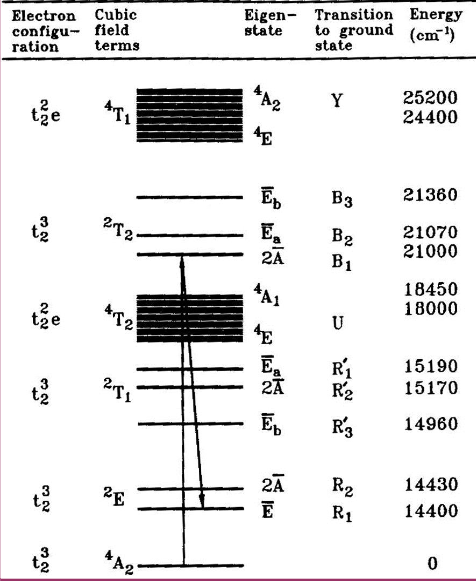
\includegraphics[width=0.3\textwidth]{./fig.png}
        \caption{$Cr^{3+}$离子参与激光作用的能级结构}
    \end{minipage}
\end{figure}


\section{结论}

\begin{enumerate}
    \item 于光栅单色仪定标的时候需要考虑到采样点是离散的这一事实,离散的采样点使得峰值可能的取值位于一个区间内。
    \item 钠灯主线系的峰值有590.025nm和596.025nm;锐线系的峰值有615.4nm和616.075nm;漫线系的峰值有
    568.25nm和568.8375nm,497.8nm和498.25nm。
    \item 计算的里德伯常数大致位于$1.13 \times 10^{-7} m^{-1}$左右,但实际值为$R = 1.09737 \times 10^{-7} m^{-1}$,可能的原因是理论模型有所偏差。
    \item 红宝石的发射光谱峰值有692.875nm和694.2875nm;其吸收光谱的峰值中心位于406.2nm和555.6nm处,其峰值带宽为100nm左右。
\end{enumerate}

\section{思考题}   

\subsection{如何求出入射狭缝的最佳宽度?}

若狭缝过宽,则衍射现象不明显;若狭缝过窄,则光强娇弱。考虑最佳宽度,在保障衍射现象的前提下,尽可能的提高光强。
这里给出一个宽度的上限。
考虑锐利判据,得:

\begin{equation}
    a_{max} = \frac{1.22\lambda f}{D}
\end{equation}

但要考虑一个最佳值的话,还需要大量的演算和实验中的验证,这里不展开。

\subsection{单色仪的理论分辨本领如何计算?怎样测量单色仪的实际分辨本领?}

理论分辨本领:

\begin{equation}
    R = \frac{\lambda}{\Delta \lambda} = \frac{Nd}{\lambda} (\sin{\theta_0}+\sin{\theta_{m}}) = mN
\end{equation}

其中m为级数,N为光栅总数。

实际分辨本领:

\begin{equation}
    R' = \frac{\lambda}{\Delta \lambda} \cong \frac{\lambda_1+\lambda_2}{2(\lambda_2-\lambda_1)}
\end{equation}

其中$\lambda_1,\lambda_2$为测量2个脉冲型光谱的中心波长。

\subsection{比较单色仪的理论分辨本领和实际分辨本领,说明两者差别大的原因。}

在实际过程中,由于环境中的光学噪声,光学器件自身的误差以及长时间工作产生热量对电信号的干扰都会影响结果。
然而,最主要的是狭缝的宽度无法准确的选取(可能导致衍射效应过于弱),以及无法有效使用所有的光栅单元,从而导致单色仪实际分辨本领比理论值小。

\subsection{解释光电倍增管的工作原理,为什么随着副高压的绝对值越大,采集的灵敏度会
显著提高?}

光电倍增管利用光电效应,用光子将电子打出,从而将光信号传唤为电信号。当负高压绝对值越大时,电子越容易
被打出,故采集的灵敏度会显著提高。

\subsection{说明溴钨灯、钠灯和汞灯的光谱的区别和道理?}

溴钨灯的光谱谱线十分的宽,从300nm到2500nm,而钠灯和汞灯则为线状分立光谱,只有几个峰值。

原因是:溴钨灯是高温固体辐射,为黑体辐射,谱线范围广;而钠灯和汞灯为高温气体发热,由于气体较为纯净,所以发出的光谱为线状的。

\section{致谢}

感谢一教物理实验中心提供的光栅单色仪以及相应的仪器,也感谢王中平老师的指导!

% 参考文献

\bibliography{math}

% 结束文档

\end{document}